\documentclass[12]{article}
\usepackage{prettyref}
\usepackage[left=2cm,right=2cm,top=2cm,bottom=2cm]{geometry}
\usepackage{graphicx}
\usepackage{amsmath, amssymb}
\usepackage{mathtools}
\usepackage{physics}
\usepackage{textcomp}
\usepackage{float}
\usepackage[british]{babel}
\usepackage{hhline}
\usepackage{multirow}
\usepackage{hyperref}
\hypersetup{
    colorlinks=true,
    linkcolor=blue,
    filecolor=magenta,      
    urlcolor=cyan,
}
\begin{document}
\begin{center}
\begin{Huge}
RESULTS-Ferromagnetic Trigger
\end{Huge}
\end{center}
%\chapter{Results}\label{ch:F}
As mentioned previously, there are two trigger Hamiltonians that were studied in the course of this thesis. This chapter focuses on the performance of quantum annealing on adding the ferromagnetic trigger, $H_T^F$ to the Hamiltonian. \\
For the same transverse-field initial Hamiltonian, and each problem from the set of problem Hamiltonians (1000 12-spin SAT problems, and 91 8-spin SAT problems), ferromagnetic trigger was added to the Hamiltonian, with three different strengths, i.e. the strength parameter, g in equation (\ref{eq:n23}) was chosen to be 0.5, 1 and 2.\\
In the subsequent sections, the effect of adding the ferromagnetic trigger with different strengths will be discussed. For studying the dynamics during the evolution, same cases have been chosen as in Chapter Original Results, so that the results can be directly compared. 

The first Hamiltonian considered in the previous chapter had high success probability (in the absence of any triggers). Figures (\ref{fig:f1}),(\ref{fig:f2}) and (\ref{fig:f3}) show the energy spectra for this case upon adding the ferromagnetic trigger with strengths 0.5, 1 and 2 respectively. The corresponding instantaneous energy values have also been included in these figures. 
\begin{figure}[H]
\centering 
\includegraphics[scale=0.3]{733_s12_F_g0.png}
\caption{The energy spectrum for the first problem, with instantaneous energy values corresponding to three annealing times, with Ferromagnetic trigger, and g=0.5. $\Delta_{min}$ was found to be 0.5779, while $p$=0.9996 for $T_A$=100. }
\label{fig:f1}
\end{figure}
\begin{figure}[H]
\centering 
\includegraphics[scale=0.3]{733_s12_F_g1.png}
\caption{The energy spectrum for the first problem, with instantaneous energy values corresponding to three annealing times, with Ferromagnetic trigger, and g=1. $\Delta_{min}$ was found to be 0.6908, while $p$=0.9998 for $T_A$=100.}
\label{fig:f2}
\end{figure}
\begin{figure}[H]
\centering 
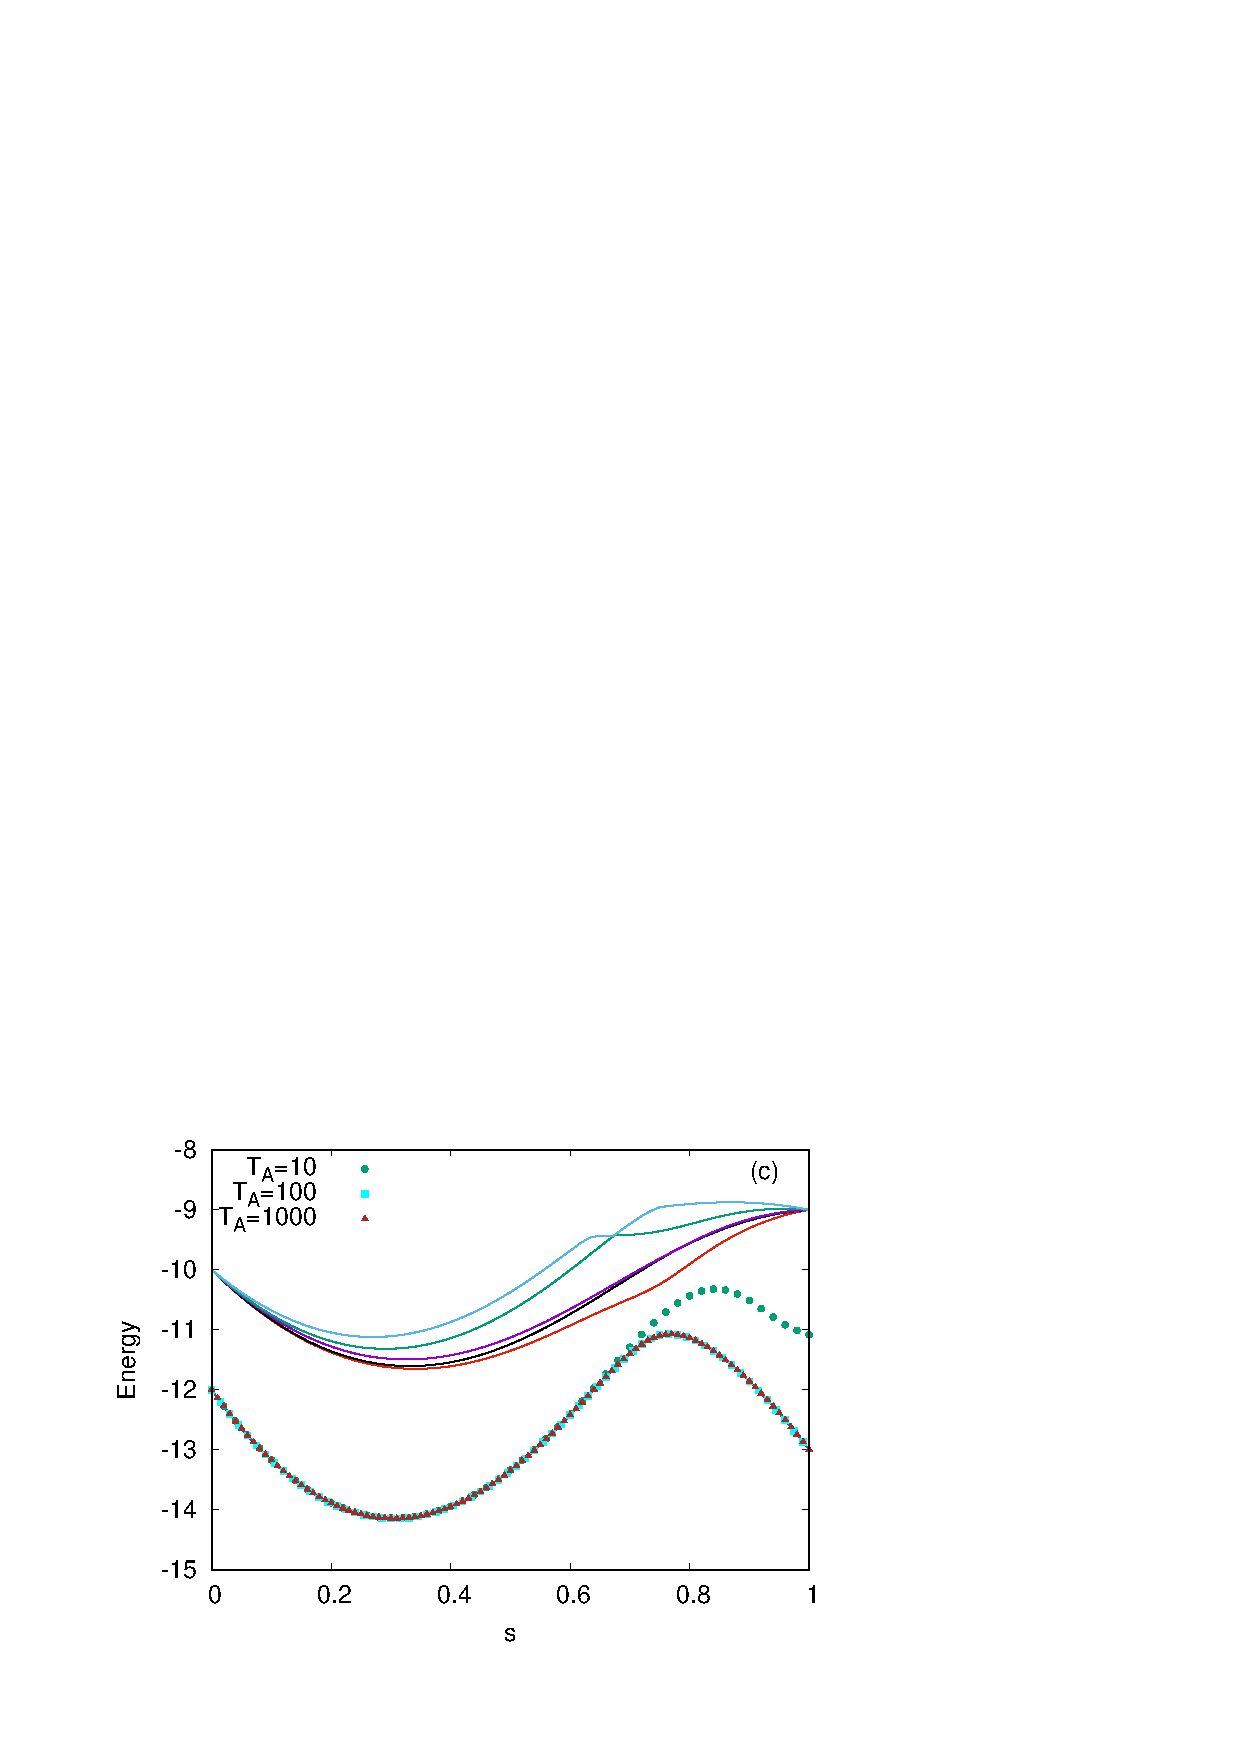
\includegraphics[scale=0.3]{733_s12_F_g2.png}
\caption{The energy spectrum for the first problem, with instantaneous energy values corresponding to three annealing times, with Ferromagnetic trigger, and g=2. $\Delta_{min}$ was found to be 0.8333, while $p$=0.9997 for $T_A$=100.}
\label{fig:f3}
\end{figure}
From these figures, it can be noted that compared to the original Hamiltonian, the minimum gap, $\Delta_{min}$ has increased for all the three case. Furthermore, the $\Delta_{min}$ becomes larger as the strength of the trigger Hamiltonian is increased from 0.5 to 2. \\
Secondly, the position of $\Delta_{min}$ is shifted more towards the right upon increasing the strength. Additionally, the concavity of the ground state also increases with it. 
Finally, all the success probabilities upon adding the trigger are larger than the success probability of the original case, owing to the increase in the the minimum gaps. Therefore, in general, the success probability also increases with increasing the strength of the trigger, though the final overlap also depends on the characteristics of the higher energy levels. 
Table (\ref{tab:f1}) shows a comparison of the minimum gaps and success probabilities between the first problem with triggers of different strengths and the original problem. 
\begin{table}
\centering
\renewcommand{\arraystretch}{1.8}
\begin{tabular}{|c|c|c|c|c|}
\hline 
Case 1 & Original Hamiltonian & g=0.5 & g=1 & g=2 \\ 
\hline 
$\Delta_{min}$ & 0.4407 & 0.5779 & 0.6908 & 0.8333 \\ 
\hline 
p & 0.9944 & 0.9996 & 0.9998 & 0.9997 \\ 
\hline 
s value at $\Delta_{min}$ & 0.459 & 0.552 & 0.629 & 0.733 \\
\hline

\end{tabular} 
\caption{A comparison of the minimum gaps and the success probabilities at $T_A$=100 for the first chosen case, between the original Hamiltonian and and the Hamiltonian with ferromagnetic trigger of different strengths. The minimum gaps become larger as the strength of the ferromagnetic trigger is increased. The success probabilities are increased as a result. The value of s corresponding to the position of the minimum gap also becomes larger.}
\label{tab:f1}
\end{table}
\textbf{Note that the success probability upon adding ferromagnetic trigger with g=2 is marginally small than that with g=1. This can be explained on the basis of}


Focussing now on the second case, which had small success probability with the original Hamiltonian, figures (\ref{fig:f4}), (\ref{fig:f5}), (\ref{fig:f6}) show the energy spectra and the instantaneous energy values of the problem upon adding the ferromagnetic trigger with g=0.5, 1 and 2 respectively. 
\begin{figure}[H]
\centering 
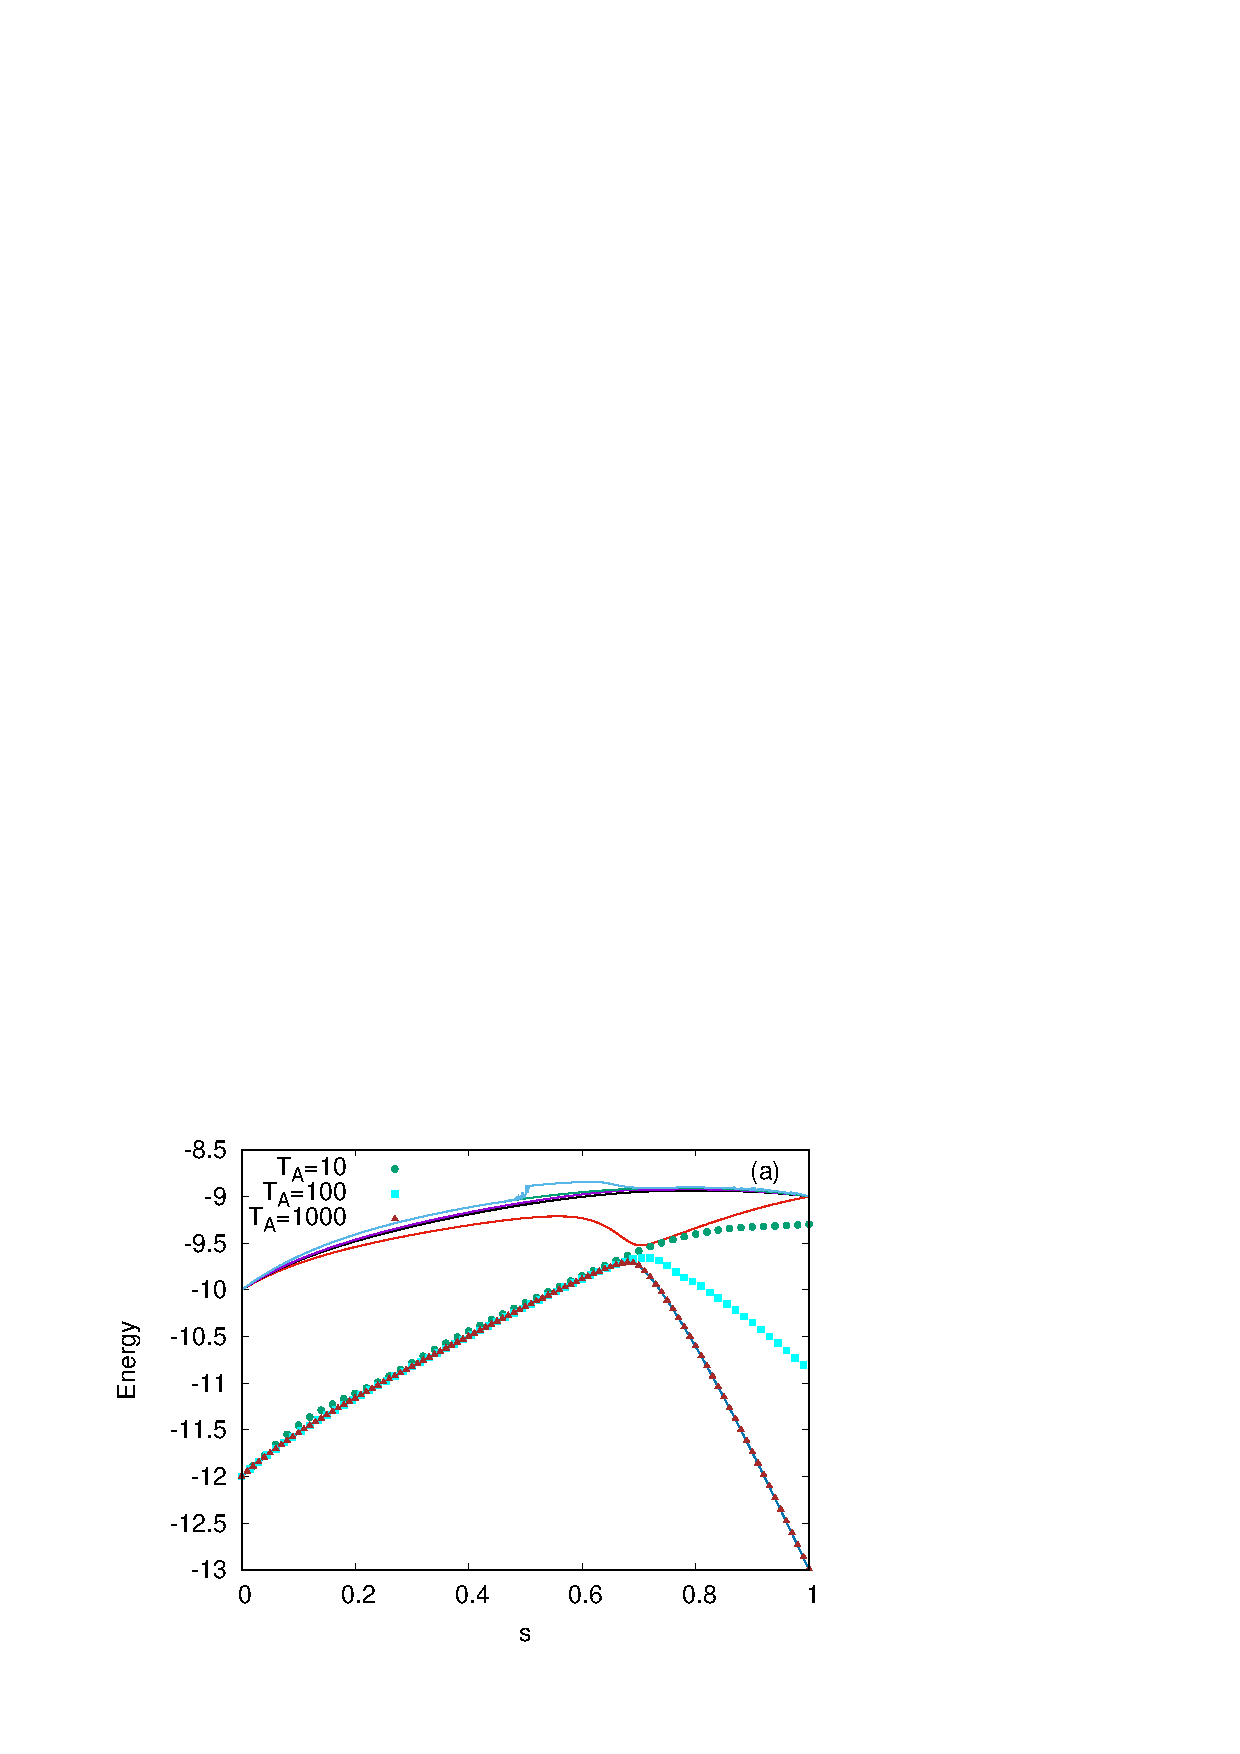
\includegraphics[scale=0.3]{950_s12_F_g0.png}
\caption{The energy spectrum for the second problem, with instantaneous energy values corresponding to three annealing times, with Ferromagnetic trigger, and g=0.5. $\Delta_{min}$ was found to be 0.2074, while $p$=0.4650 for $T_A$=100.}
\label{fig:f4}
\end{figure}
For this case too, the minimum energy gaps were found to have increased, leading to an improvement in the success probabilities. The improvements can be seen to become larger with increasing strengths of the trigger. The position of the minimum gap was again found to shift more rightwards in terms of the annealing parameter s upon increasing the strength. \\
\begin{figure}[H]
\centering 
\includegraphics[scale=0.3]{950_s12_F_g1.png}
\caption{The energy spectrum for the second problem, with instantaneous energy values corresponding to three annealing times, with Ferromagnetic trigger, and g=1. $\Delta_{min}$ was found to be 0.4129, while $p$=0.8889 for $T_A$=100.}
\label{fig:f5}
\end{figure}
\begin{figure}[H]
\centering 
\includegraphics[scale=0.3]{950_s12_F_g2.png}
\caption{The energy spectrum for the second problem, with instantaneous energy values corresponding to three annealing times, with Ferromagnetic trigger, and g=2. $\Delta_{min}$ was found to be 0.6943, while $p$=0.9870 for $T_A$=100.}
\label{fig:f6}
\end{figure}


One feature of difference, however, compared to the first case was the factor by which the success probability is improved upon adding the ferromagnetic trigger to the original Hamiltonian. For the second case,$T_A$=100, and g=2, the ratio of the success probabilities upon adding the ferromagnetic trigger ($p^F$) to the original success probability ($p^O$), is $\dfrac{p^F}{p^O}$=67.6. In terms of the ratio of the corresponding minimum gaps this improvement was $\dfrac{\Delta_{min}^F}{\Delta_{min}^O}$=22.2. On the other hand, for the first chosen case, $\dfrac{p^F}{p^O}$=1.005, whereas $\dfrac{\Delta_{min}^F}{\Delta_{min}^O}$=1.89 for g=2. Since for the first case, the instantaneous state lies close to the ground state even for the original Hamiltonian (figure \ref{fig:o2}), adding the trigger cannot do much improvement. On the contrary, since for the second case the minimum gap is comparatively very small, the instantaneous state comes close to the first excited state upon approaching the minimum energy anti-crossing. Adding the ferromagnetic trigger can then open this gap so that the system state always stays close to the ground state. This can explain the difference in the improvement ratios for the two cases.

Table (\ref{tab:f2}) gives the comparison of the minimum gaps and the success probabilities for $T_A$=100 for this case, between the original Hamiltonian and upon adding ferromagnetic triggers with different strengths.
\begin{table}
\centering
\renewcommand{\arraystretch}{1.8}
\begin{tabular}{|c|c|c|c|c|}
\hline 
Case 2 & Original Hamiltonian & g=0.5 & g=1 & g=2 \\ 
\hline 
$\Delta_{min}$ & 0.0312 & 0.2074 & 0.4129 & 0.6943 \\ 
\hline 
p & 0.0146 & 0.4650 & 0.8889 & 0.9870 \\ 
\hline 
s value at $\Delta_{min}$ & 0.665 & 0.691 & 0.727 & 0.793 \\
\hline

\end{tabular} 
\caption{A comparison of the minimum gaps and the success probabilities at $T_A$=100 for the second chosen case, between the original Hamiltonian and and the Hamiltonian with ferromagnetic trigger of different strengths. The minimum gaps become larger as the strength of the ferromagnetic trigger is increased. The success probabilities are increased as a result. The value of s corresponding to the position of the minimum gap also becomes larger.}
\label{tab:f2}
\end{table}

Next, we consider the third case of intermediate success probability with original Hamiltonian. Figures (\ref{fig:f7}), (\ref{fig:f8}) and (\ref{fig:f9}) show the energy spectra and the instantaneous energy values after adding the ferromagnetic trigger with strengths 0.5, 1 and 2 respectively.
\begin{figure}[H]
\centering 
\includegraphics[scale=0.3]{528_s12_F_g0.png}
\caption{The energy spectrum for the third problem, with instantaneous energy values corresponding to three annealing times, with Ferromagnetic trigger, and g=0.5. $\Delta_{min}$ was found to be 0.3748, while $p$=0.9577 for $T_A$=100.}
\label{fig:f7}
\end{figure}
For this case too, the minimum energy gaps were found to have increased, leading to an improvement in the success probabilities. The improvements can be seen to become larger with increasing strengths of the trigger. The position of the minimum gap was again found to shift more rightwards in terms of the annealing parameter s upon increasing the strength. \\
\begin{figure}[H]
\centering 
\includegraphics[scale=0.3]{528_s12_F_g1.png}
\caption{The energy spectrum for the third problem, with instantaneous energy values corresponding to three annealing times, with Ferromagnetic trigger, and g=1. $\Delta_{min}$ was found to be 0.5439, while $p$=0.9945 for $T_A$=100.}
\label{fig:f8}
\end{figure}
\begin{figure}[H]
\centering 
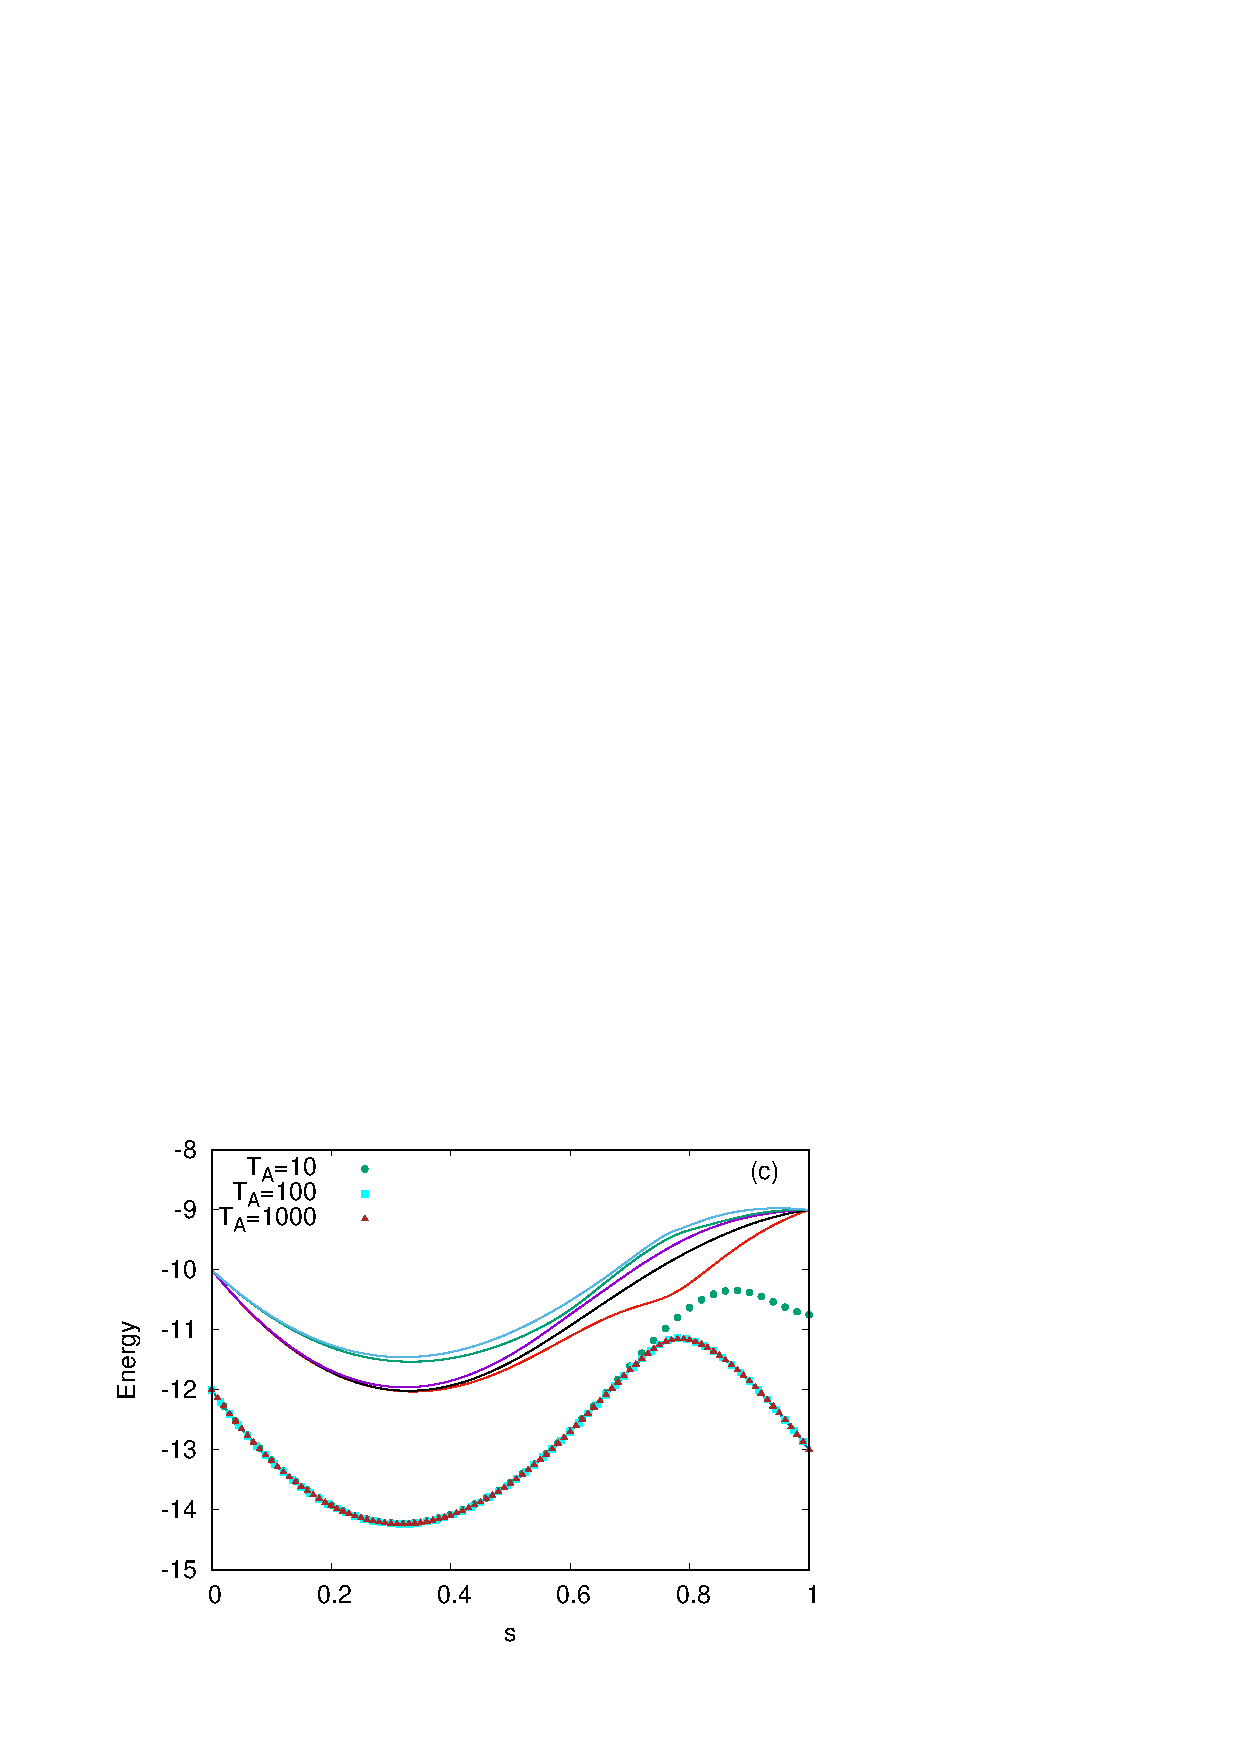
\includegraphics[scale=0.3]{528_s12_F_g2.png}
\caption{The energy spectrum for the third problem, with instantaneous energy values corresponding to three annealing times, with Ferromagnetic trigger, and g=2. $\Delta_{min}$ was found to be 0.7512, while $p$=0.9981 for $T_A$=100.}
\label{fig:f9}
\end{figure}
The improvement ratio for this case,$\dfrac{p^F}{p^O}$=1.91 , while $\dfrac{\Delta_{min}^F}{\Delta_{min}^O}$=4.77 at g=2. These values also are intermediate to those for the first and the second case.  Table (\ref{tab:f3}) shows a comparison of the success probabilities and the minimum gaps, between the original Hamiltonian and after adding the ferromagnetic trigger with different strengths.
\begin{table}
\centering
\renewcommand{\arraystretch}{1.8}
\begin{tabular}{|c|c|c|c|c|}
\hline 
Case 3 & Original Hamiltonian & g=0.5 & g=1 & g=2 \\ 
\hline 
$\Delta_{min}$ & 0.1573 & 0.3748 & 0.5439 & 0.7512 \\ 
\hline 
p & 0.5199 & 0.9577 & 0.9945 & 0.9981 \\ 
\hline 
s value at $\Delta_{min}$ & 0.514 & 0.595 & 0.665 & 0.760 \\
\hline

\end{tabular} 
\caption{A comparison of the minimum gaps and the success probabilities at $T_A$=100 for the third chosen case, between the original Hamiltonian and and the Hamiltonian with ferromagnetic trigger of different strengths. The minimum gaps become larger as the strength of the ferromagnetic trigger is increased. The success probabilities are increased as a result. The value of s corresponding to the position of the minimum gap also becomes larger.}
\label{tab:f3}
\end{table}
Next, the minimum gaps and the success probabilities were computed for all the problems belonging to 12-SAT problems, before and after adding the ferromagnetic trigger, with g $\in$ \{0.5,1,2\}, for $T_A$ $\in$ {10,100,1000}. \\

Figure (\ref{fig:f10}) shows the scatter plot of the original minimum energy gaps with the corresponding minimum energy gaps upon adding the ferromagnetic trigger with different strengths, for all the problems of the set.

\begin{figure}[H]
\centering 
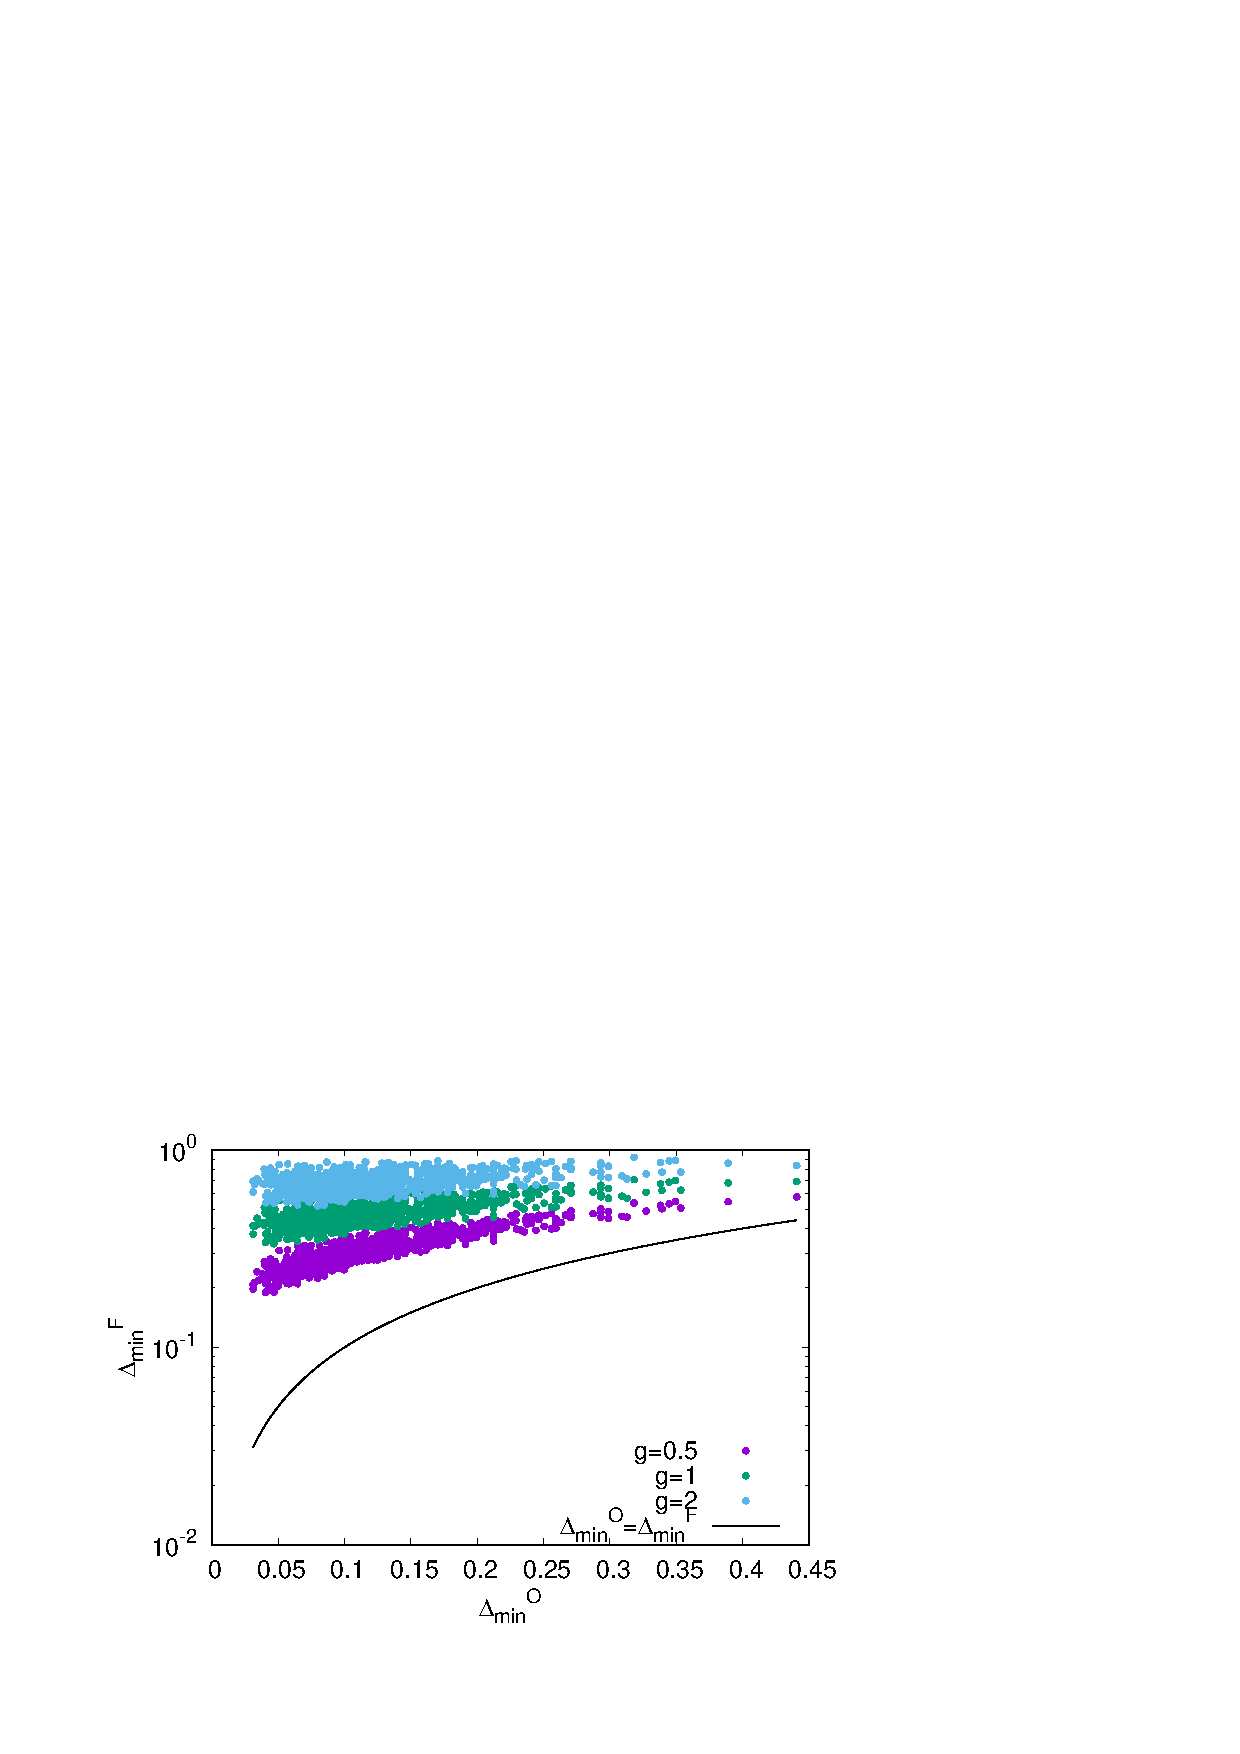
\includegraphics[scale=0.25]{Mingap_F_g0_1_2.png}
\caption{Scatter plot of the minimum gaps of the original Hamiltonians with those upon adding the ferromagnetic trigger with g $\in$ \{0.5,1,2\}. The solid line represents the region where the minimum gap remains unchanged.}
\label{fig:f10}
\end{figure}
With ferromagnetic trigger, all the minimum gaps were found to have increased, for  the three strengths of the trigger. Furthermore, for all the problems, the gaps became larger, as the ferromagnetic trigger became stronger, and the distribution of points can be noted to be quite systematic. As explained previously in terms of the improvement ratios of the first and the second chosen cases, the improvement for harder cases (small minimum gaps) is much larger than the improvement for easier cases (large minimum gaps).

For gauging the performance of the Hamiltonian after adding the ferromagnetic triggers, scatter plots of the original success probability with that obtained upon adding the trigger have been shown in figure (\ref{fig:f11}), (\ref{fig:f12}) and (\ref{fig:f13}) corresponding to g= 0.5, 1 and 2 respectively.
\begin{figure}[H]
\centering 
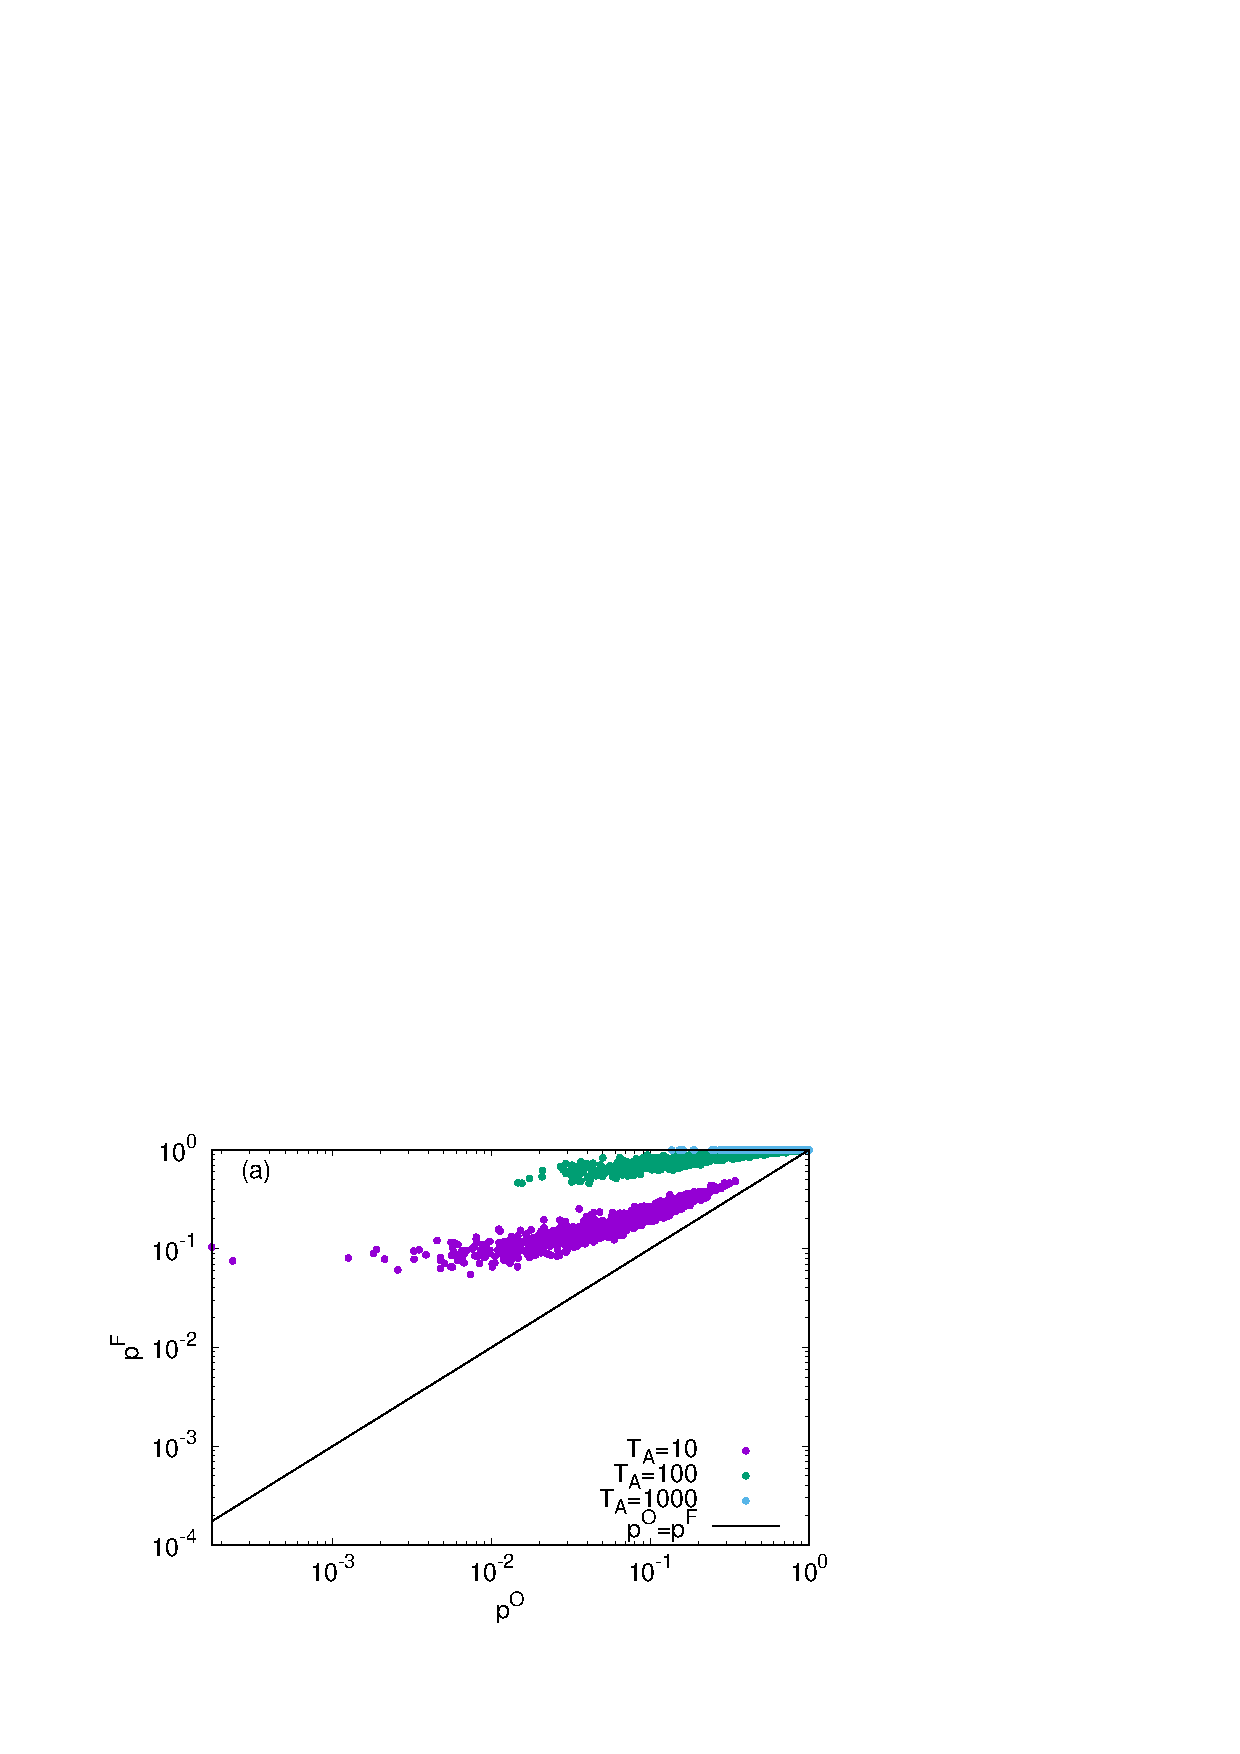
\includegraphics[scale=0.3]{Scatt_s12_F_g0.png}
\caption{Scatter plot for the success probability after adding ferromagnetic trigger with the success probability of the original Hamiltonian, for annealing time $T_A \in \{10,100,1000\}$. The solid line represents the region where the success probability remains unchanged.}
\label{fig:f11}
\end{figure}
\begin{figure}[H]
\centering
\includegraphics[scale=0.3]{Scatt_s12_F_g1.png}
\caption{Scatter plot for the success probability after adding ferromagnetic trigger with the success probability of the original Hamiltonian, for annealing time $T_A \in \{10,100,1000\}$. The solid line represents the region where the success probability remains unchanged.}
\label{fig:f12}
\end{figure}
\begin{figure}[H]
\centering
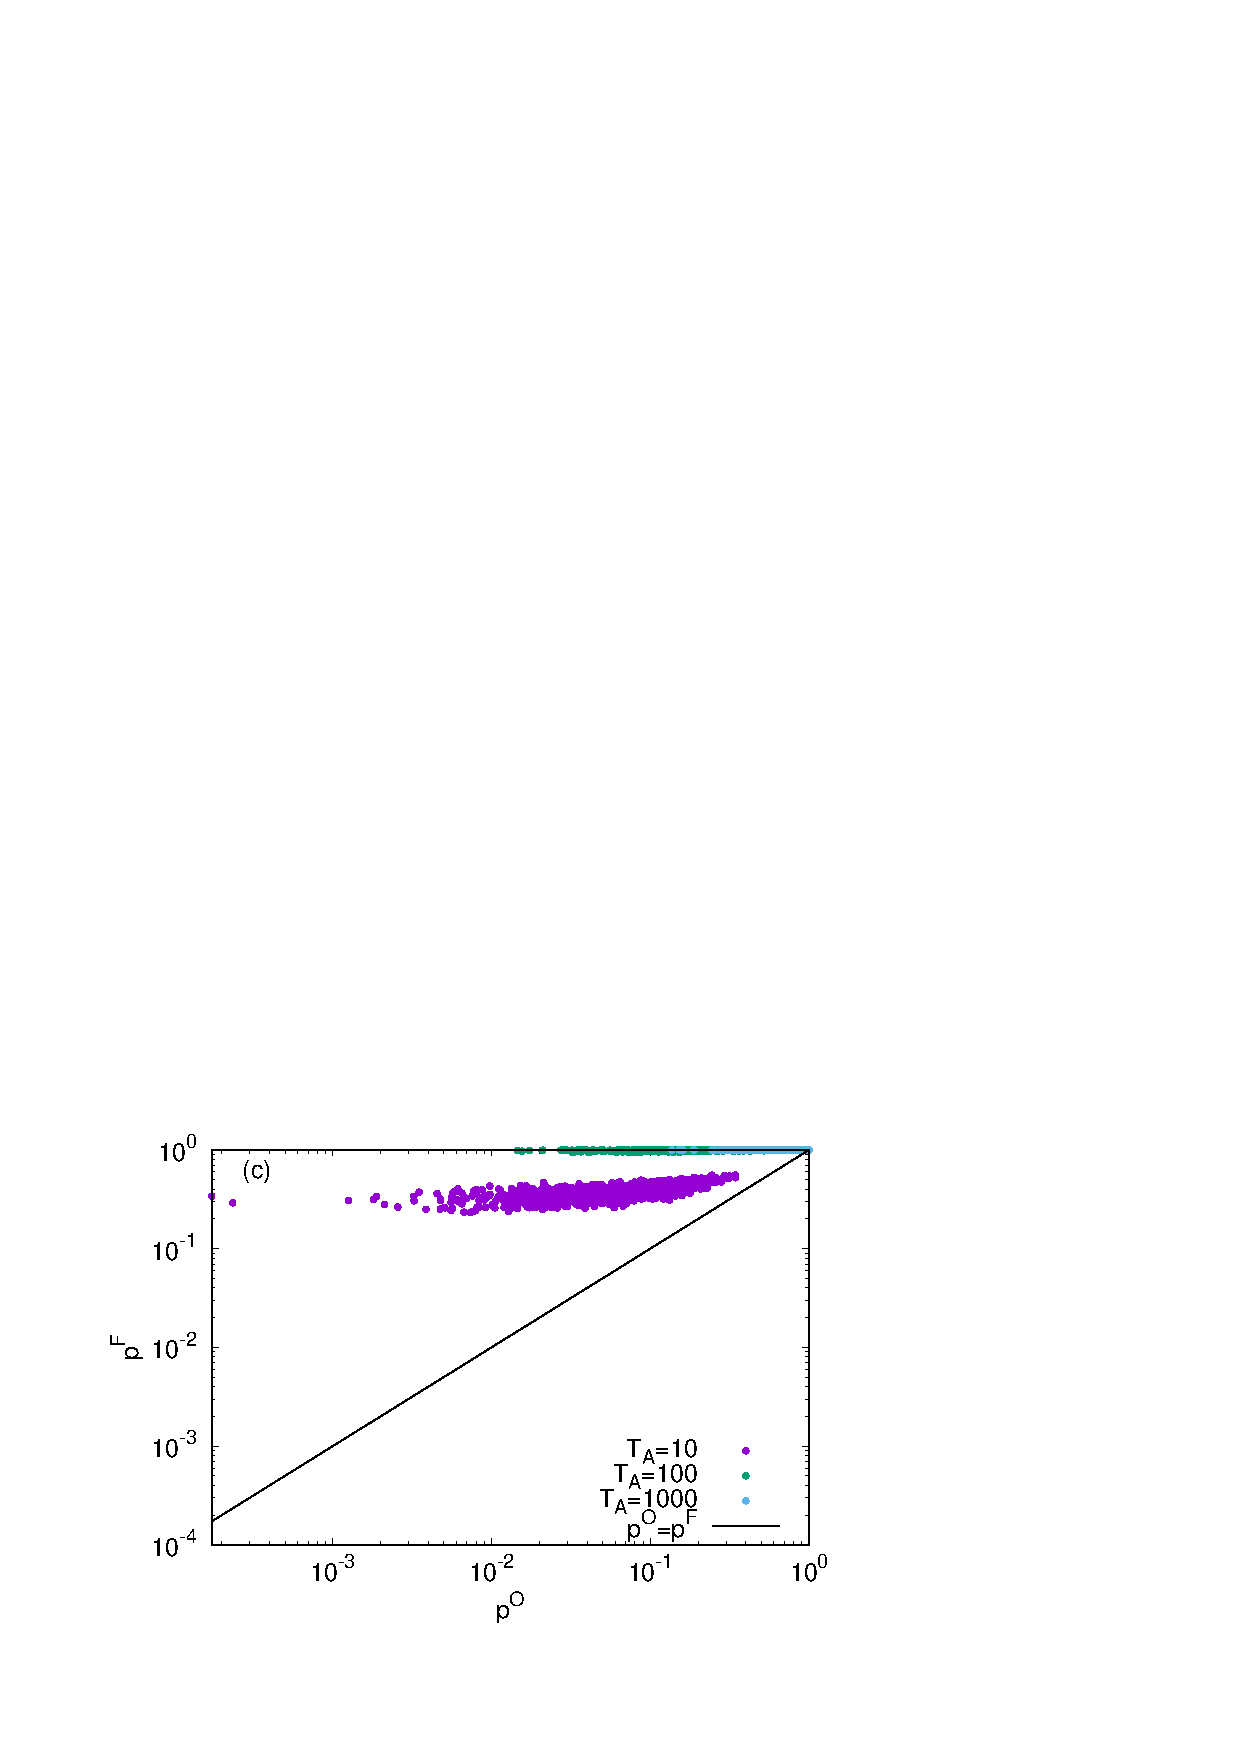
\includegraphics[scale=0.3]{Scatt_s12_F_g2.png}
\caption{Scatter plot for the success probability after adding ferromagnetic trigger with the success probability of the original Hamiltonian, for annealing time $T_A \in \{10,100,1000\}$. The solid line represents the region where the success probability remains unchanged.}
\label{fig:f13}
\end{figure}

For all the three cases, and all the problems in the set, the success probability after adding the trigger was found to be greater than the success probability of the original Hamiltonian. Since in the adiabatic regime, the overlap of the final state with the ground state increases with increasing the annealing times, the success probability of the original Hamiltonians with long annealing times ($T_A$=1000) is already large ($\approx$ 1). Adding the ferromagnetic trigger can therefore not improve the success probability too much. This explains the confinement of $T_A$=1000 points close to the solid line ($p^O=p^F$) on the upper right corner for all the three values of the strength parameter. Owing to the same reason, the points corresponding to $T_A$=10 have a much larger spread. For the easy cases (larger $p^O$), the success probability upon adding the trigger ($p^F$) has a similar value. Such points lie close to the line. On the other hand, for the more difficult cases (smaller $p^O$) the improvement can be larger, and such points lie away from the line.\\

Furthermore, since for a given problem, increasing the strength of the ferromagnetic trigger makes the minimum gap larger, the success probability for that case also becomes larger. This explains the distribution of the points getting successively more flat with increasing strength of the trigger, for all annealing times (compare figures \ref{fig:f11}, \ref{fig:f12} and \ref{fig:f13}).\\

Finally, we look at the dynamics of the evolution. According to equation (\ref{eq:lz3}), for an adiabatic evolution of the state of the system, the success probability, p, i.e. the measure of the overlap of the final state with the ground state of the Hamiltonian, is related to the minimum energy gap, $\Delta_{min}$ as follows:
\begin{equation}
p=1-exp(-C{\Delta_{min}}^2),
\end{equation}
for some constant C. Since different problems in the problem set correspond to different minimum energy gaps, a plot of the success probability with these gaps should follow equation (\ref{eq:lz3}) if the evolution of the state for a problem is adiabatic. Moreover, adding the trigger changes the energy spectra, and thereby the minimum energy gaps of these problems. Figure (\ref{fig:f14}) shows the success probability versus the minimum energy gap plot for all the problems, and the upon adding the ferromagnetic trigger with three different strengths (0.5,1 and 2), and for three annealing times (10,100 and 1000).

\begin{figure}[H]
\centering
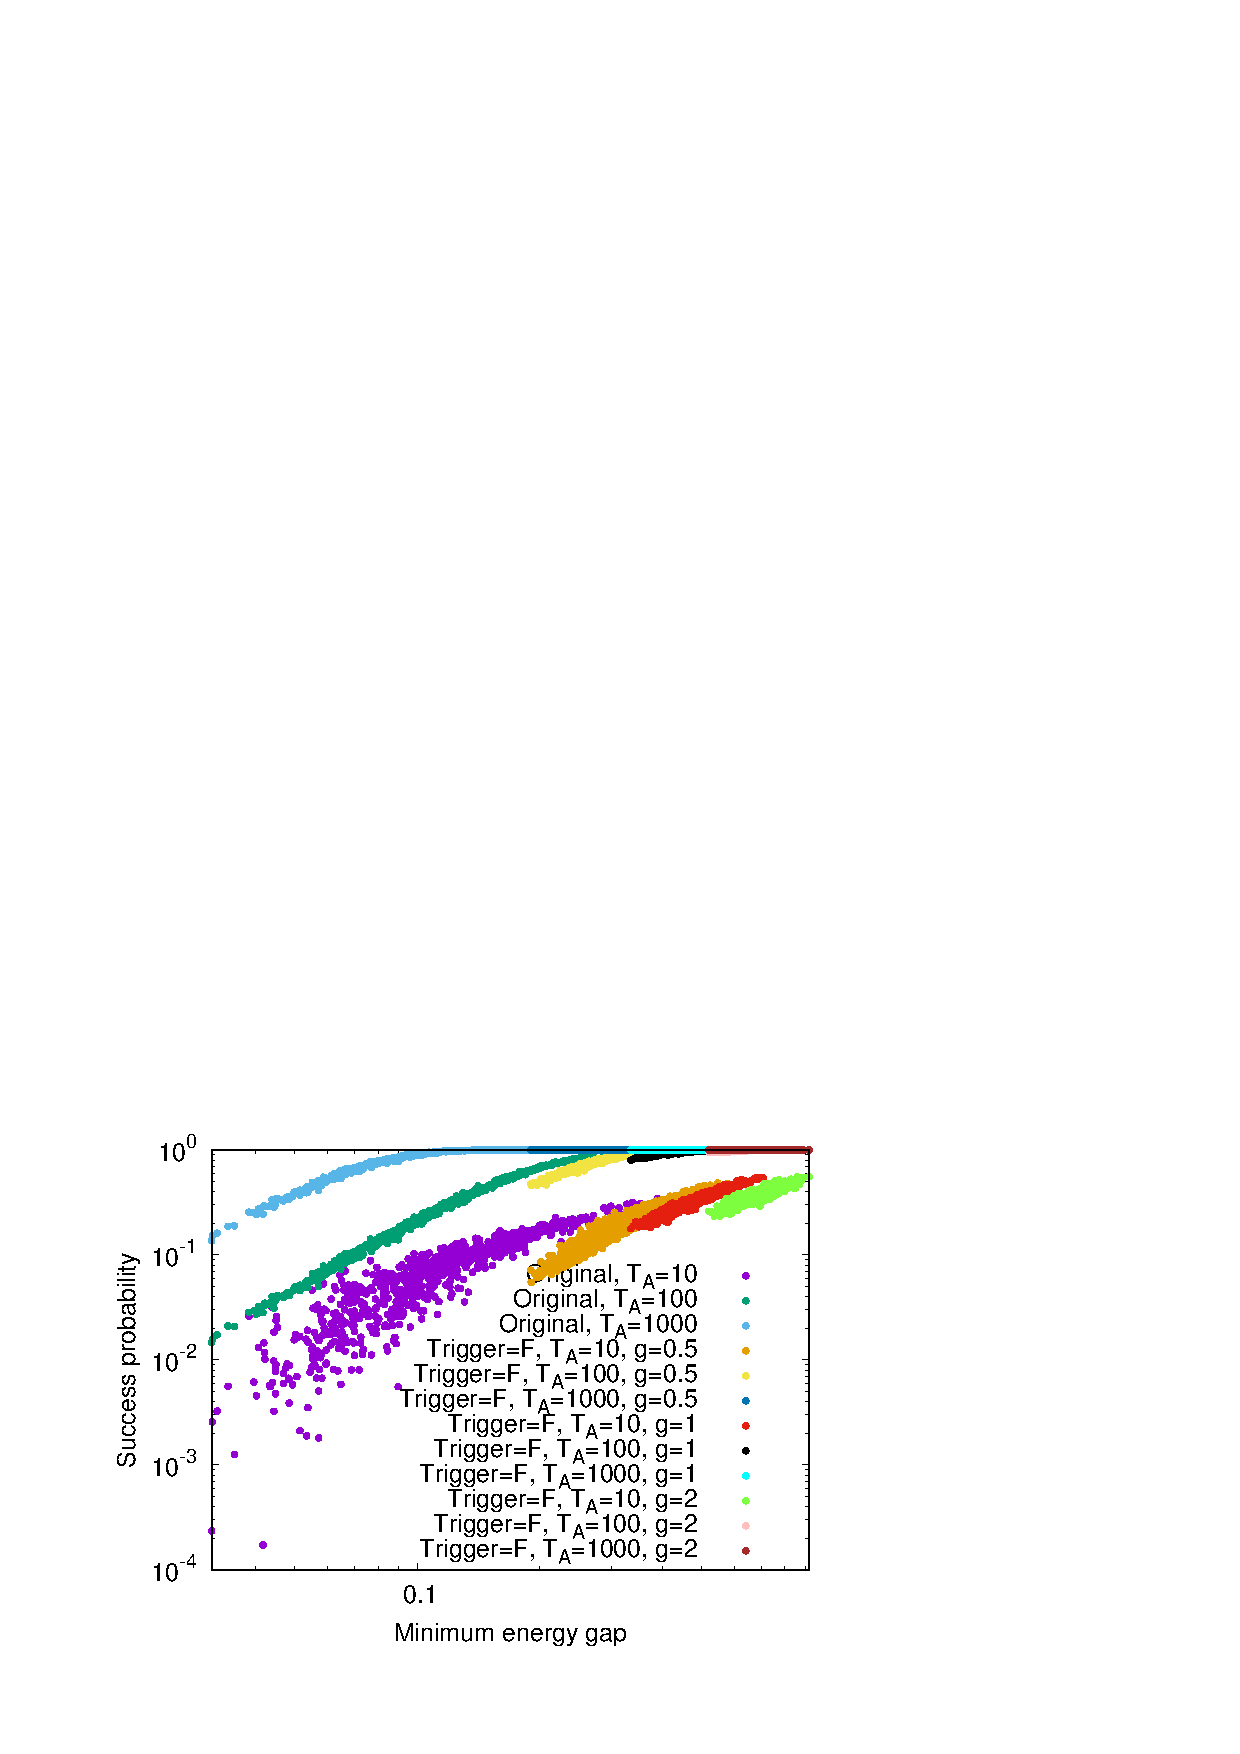
\includegraphics[scale=0.3]{SuccVsGap_OF_g.png}
\caption{Plot of success probability versus the minimum energy gaps for all the problems belonging to the set. The plot the effect of adding ferromagnetic trigger to the original Hamiltonian with strengths 0.5, 1 and 2, while the annealing time is chosen to 10, 100 and 1000.}
\label{fig:f14}
\end{figure} 

From the figure (\ref{fig:f14}) it can be noted that all the curves roughly follow the exponential  relation of equation (\ref{eq:lz3}). However, for the original Hamiltonian, and $T_A$=10, the scattering is quite larger compared to the other curves. The scattering of the curves decreases on increasing the annealing times, suggesting that longer annealing times ascertain the evolution of the state to be adiabatic. Since adding the ferromagnetic trigger enlarges the minimum energy gaps, the curves are shifted to the right upon adding the trigger and increasing their strength. 
\end{document}